\begin{figure}[htbp]
\centering
\resizebox{\textwidth}{!}{%
	\begin{tikzpicture}[
		trave/.style  = {line width=2.0pt, line cap=round, line join=round, black},
		terra/.style  = {line width=0.8pt, black},
		fibra/.style  = {line width=0.65pt, dashed, gray!55, line cap=round},
		carr/.style   = {->, >=stealth, line width=1.0pt, black},
		diag/.style   = {line width=0.9pt, black},
		nodo/.style   = {circle, fill=white, draw=black,
			inner sep=0pt, minimum size=5pt, line width=0.8pt},
		cint/.style   = {circle, fill=white, draw=black,
			inner sep=0pt, minimum size=6.5pt, line width=1.0pt},
		segno/.style  = {circle, draw=black, fill=white, inner sep=0pt,
			minimum size=9pt, font=\tiny, line width=0.55pt},
		lab/.style    = {font=\small},
		tlab/.style   = {font=\small},
		]
		
		%% ── Parametri ────────────────────────────────────────────────────────────
		\def\Ls{1.80}
		\def\twi{0.20}  \def\thA{0.38}  \def\thR{0.30}
		\def\bww{0.13}  \def\gww{0.26}
		
		\def\TA{0.72}   \def\TB{0.28}   \def\TC{0.54}   % T_0
		\def\Ts{0.52}                                    % T_1, T_2
		\def\MA{1.00}   \def\MB{0.80}   \def\MC{0.65}   % M_0
		\def\Ms{1.05}                                    % M_1, M_2 (vertice)
		
		%% ── Macro vincoli ────────────────────────────────────────────────────────
		\newcommand{\cernieraA}{%
			\draw[terra](0,0)--++(-\twi,-\thA)--++(2*\twi,0)--cycle;
			\draw[terra]({-\gww},{-\thA})--(\gww,{-\thA});
			\foreach \xi in {-0.20,-0.10,0.00,0.10,0.20}
			\draw[very thin,black](\xi,{-\thA})--++(-0.09,-0.11);
			\node[nodo]at(0,0){};}
		
		\newcommand{\carrello}[1]{%
			\draw[terra](#1,0)--++(-\twi,-\thR)--++(2*\twi,0)--cycle;
			\draw[terra]({#1-\gww},{-\thR})--({#1+\gww},{-\thR});
			\draw[terra]({#1-\bww},{-\thR-0.13})circle(2.0pt);
			\draw[terra]({#1+\bww},{-\thR-0.13})circle(2.0pt);
			\draw[terra]({#1-\gww},{-\thR-0.26})--({#1+\gww},{-\thR-0.26});
			\foreach \xi in {-0.20,-0.10,0.00,0.10,0.20}
			\draw[very thin,black]({#1+\xi},{-\thR-0.26})--++(-0.09,-0.11);
			\node[nodo]at(#1,0){};}
		
		\newcommand{\traveVincoli}{%
			\draw[trave](0,0)--({3*\Ls},0);
			\cernieraA
			\carrello{\Ls}  \carrello{2*\Ls}  \carrello{3*\Ls}}
		
		%% Label nodi standard (above=0.04 per tutti)
		\newcommand{\nodiABCD}{%
			\node[lab,above=0.04]at(0,0){$A$};
			\node[lab,above=0.04]at({\Ls},0){$B$};
			\node[lab,above=0.04]at({2*\Ls},0){$C$};
			\node[lab,above=0.04]at({3*\Ls},0){$D$};}
		
		\newcommand{\traveVincoliCI}{%
			\traveVincoli
			\node[cint]at({\Ls},0){};
			\node[cint]at({2*\Ls},0){};}
		
		\newcommand{\fibraInf}{%
			\draw[fibra](0,-0.15)--({3*\Ls},-0.15);}
		
		%% ── Intestazioni di colonna ──────────────────────────────────────────────
		\node[lab,align=center]at({0.5*3*1.80},     1.10){\textbf{Problema 0}};
		\node[lab,align=center]at({7.0+0.5*3*1.80}, 1.10){\textbf{Problema 1}};
		\node[lab,align=center]at({14.0+0.5*3*1.80},1.10){\textbf{Problema 2}};
		
		%% ════════════════════════════════════════════════════════════════════════
		%% COLONNA 1 — Problema 0
		%% ════════════════════════════════════════════════════════════════════════
		
		%%─── (a) Schema ─────────────────────────────────────────────────────────
		\begin{scope}[xshift=0cm, yshift=0cm]
			\traveVincoliCI  \fibraInf
			%% etichette nodi (A a sinistra, B a destra)
			\node[lab,above left=0.04]at(0,0){$A$};
			\node[lab,above right=0.04]at({\Ls},0){$B$};
			\node[lab,above right=0.04]at({2*\Ls},0){$C$};
			\node[lab,above=0.04]at({3*\Ls},0){$D$};
			%% rettangolo delimitatore del carico p
			\draw[black,line width=0.5pt](0,0.07)--(0,0.52)--({1.80},0.52)--({1.80},0.07);
			\foreach \k in {0,1,2,3,4,5,6}{
				\pgfmathsetmacro{\xk}{\k*(1.80/6.0)}
				\draw[carr]({\xk},0.52)--({\xk},0.08);}
			\node[tlab,above]at({0.5*1.80},0.59){$p$};
			%% coppia μ in C: arco 180° CCW, convessità verso BC
			\draw[->,>=stealth,line width=0.85pt]({2*1.80},{0.24})arc(90:270:0.24);
			\node[tlab,right]at({2*1.80-0.50},0.25){$\mu$};
			\draw[carr]({2.5*1.80},0.52)--({2.5*1.80},0.07);
			\node[tlab,above]at({2.5*1.80},0.59){$F$};
			\node[lab]at({1.5*1.80},-0.95){$(a)$};
		\end{scope}
		
		%%─── (d) T_0  ──  fill → diag → struttura → etichette + cerchietti ──────
		\begin{scope}[xshift=0cm, yshift=-2.7cm]
			%% 1. fill
			\fill[gray!15](0,0)--(0,\TA)--({0.5*\Ls},0)--cycle;
			\fill[gray!15]({0.5*\Ls},0)--({\Ls},0)--({\Ls},{-\TA})--cycle;
			\fill[gray!15]({\Ls},0)rectangle({2*\Ls},\TB);
			\fill[gray!15]({2*\Ls},0)--({2*\Ls},\TC)--({2.5*\Ls},\TC)--({2.5*\Ls},0)--cycle;
			\fill[gray!15]({2.5*\Ls},0)--({2.5*\Ls},{-\TC})--({3*\Ls},{-\TC})--(3*\Ls,0)--cycle;
			%% 2. contorni diagramma
			\draw[diag](0,\TA)--({0.5*\Ls},0)--({\Ls},{-\TA});
			\draw[diag](0,0)--(0,\TA);
			\draw[diag]({\Ls},{-\TA})--({\Ls},\TB);          % salto B
			\draw[diag]({\Ls},0)--({\Ls},\TB);
			\draw[diag]({\Ls},\TB)--({2*\Ls},\TB);
			\draw[diag]({2*\Ls},0)--({2*\Ls},\TB);
			\draw[diag]({2*\Ls},\TB)--({2*\Ls},\TC);          % salto C
			\draw[diag]({2*\Ls},\TC)--({2.5*\Ls},\TC);
			\draw[diag]({2.5*\Ls},\TC)--({2.5*\Ls},{-\TC});   % gradino F
			\draw[diag]({2.5*\Ls},{-\TC})--({3*\Ls},{-\TC});
			\draw[diag]({3*\Ls},{-\TC})--({3*\Ls},0);
			%% 3. struttura (in primo piano)
			\traveVincoliCI  \fibraInf
			%\nodiABCD
			\node[lab,above left=0.04]at(0,0){$A$};
			\node[lab,above left=0.04]at({\Ls},0){$B$};
			\node[lab,above=0.04]at({2*\Ls},0){$C$};
			\node[lab,above=0.04]at({3*\Ls},0){$D$};
			
			%% 4. etichette valori
			\node[tlab,left]at(0,\TA){$\tfrac{p\ell}{2}$};
			\node[tlab,right]at({\Ls},{-\TA}){$\tfrac{p\ell}{2}$};
			\node[tlab,above]at({1.5*\Ls},\TB){$\tfrac{\mu}{\ell}$};
			\node[tlab,above]at({2.25*\Ls},\TC){$\tfrac{F}{2}$};
			\node[tlab,below]at({2.75*\Ls},{-\TC}){$\tfrac{F}{2}$};
			%% 5. cerchietti ±
			\node[segno]at({0.5*\Ls*0.35},{\TA*0.33}){$+$};   % AB sopra
			\node[segno]at({\Ls*0.85},{-\TA*0.33}){$-$};       % AB sotto
			\node[segno]at({1.5*\Ls},{\TB*0.52}){$+$};         % BC
			\node[segno]at({2.25*\Ls},{\TC*0.52}){$+$};        % CD prima metà
			\node[segno]at({2.75*\Ls},{-\TC*0.52}){$-$};       % CD seconda metà
			\node[lab]at({1.5*\Ls},-1.4){$(d)$};
		\end{scope}
		
		%%─── (g) M_0  ──  fill → diag → struttura → etichette ──────────────────
		\begin{scope}[xshift=0cm, yshift=-6.0cm]
			%% 1. fill
			\fill[gray!15](0,0)
			plot[domain=0:1,samples=22]({\x*1.80},{-1.00*4*\x*(1-\x)})--cycle;
			\fill[gray!15]({\Ls},0)--({2*\Ls},{-\MB})--({2*\Ls},0)--cycle;
			\fill[gray!15]({2*\Ls},0)--({2.5*\Ls},{-\MC})--({3*\Ls},0)--cycle;
			%% 2. contorni diagramma
			\draw[diag]plot[domain=0:1,samples=22]({\x*1.80},{-1.00*4*\x*(1-\x)});
			\draw[diag]({\Ls},0)--({2*\Ls},{-\MB});
			\draw[diag]({2*\Ls},{-\MB})--({2*\Ls},0);                              % lato dx BC
			\draw[dashed,gray!65,line width=0.70pt]({2*\Ls},{-\MB})--({2*\Ls},0); % salto C
			\draw[->,>=stealth,line width=0.55pt,gray!75]
			({2*\Ls+0.18},{-\MB*0.58})--({2*\Ls+0.18},-0.05);
			\draw[diag]({2*\Ls},0)--({2.5*\Ls},{-\MC})--({3*\Ls},0);
			%% 3. struttura
			\traveVincoliCI  \fibraInf
			\nodiABCD
			%% 4. etichette
			\node[tlab,above]at({0.5*1.80},{-\MA}){$\tfrac{p\ell^2}{8}$};
			\node[tlab,below right]at({2*\Ls},{-\MB}){$\mu$};
			%\node[tlab,right,gray!75]at({2*\Ls+0.20},{-\MB*0.55}){$\Delta M$};
			\node[tlab,above]at({2.5*\Ls},{-\MC}){$\tfrac{F\ell}{4}$};
			\node[lab]at({1.5*1.80},-0.90){$(g)$};
		\end{scope}
		
		%% ════════════════════════════════════════════════════════════════════════
		%% COLONNA 2 — Autosoluzione 1  (χ₁=1)
		%% ════════════════════════════════════════════════════════════════════════
		
		%%─── (b) Schema ─────────────────────────────────────────────────────────
		\begin{scope}[xshift=7.0cm, yshift=0cm]
			\traveVincoliCI  \fibraInf
			\nodiABCD
			%% coppia χ₁=1 in B: arco CW (sx, aperto a sx) + arco CCW (dx, aperto a dx)
			\def\rchi{0.20}   % raggio
			\def\dchi{0.20}   % offset dei centri da B  (= rchi → gli archi si sfiorano in B)
			%% SX (CW): centro a B-dchi, semicerchio sinistro, freccia in cima punta verso B
			\draw[->,>=stealth,line width=0.88pt]
			({1.80-\dchi},{-\rchi}) arc(270:90:\rchi);
			%% DX (CCW): centro a B+dchi, semicerchio destro, freccia in cima punta verso B
			\draw[->,>=stealth,line width=0.88pt]
			({1.80+\dchi},{-\rchi}) arc(-90:90:\rchi);
			\node[tlab,above=0.30]at({1.80},0){$\chi_1{=}1$};
			\node[lab]at({1.5*\Ls},-0.95){$(b)$};
		\end{scope}
		
		%%─── (e) T_1  ──  fill → diag → struttura → etichette + cerchietti ──────
		\begin{scope}[xshift=7.0cm, yshift=-2.7cm]
			%% 1. fill
			\fill[gray!15](0,0)rectangle({\Ls},\Ts);
			\fill[gray!15]({\Ls},{-\Ts})rectangle({2*\Ls},0);
			%% 2. contorni
			\draw[diag](0,0)--(0,\Ts)--({\Ls},\Ts);
			\draw[diag]({\Ls},0)--({\Ls},\Ts);
			\draw[diag]({\Ls},\Ts)--({\Ls},{-\Ts});          % salto B
			\draw[diag]({\Ls},{-\Ts})--({2*\Ls},{-\Ts});
			\draw[diag]({2*\Ls},0)--({2*\Ls},{-\Ts});
			\draw[diag]({2*\Ls},{-\Ts})--({2*\Ls},0);        % salto C
			%% 3. struttura
			\traveVincoliCI  \fibraInf
			%\nodiABCD
			\node[lab,above left=0.04]at(0,0){$A$};
			\node[lab,above right=0.04]at({\Ls},0){$B$};
			\node[lab,above=0.04]at({2*\Ls},0){$C$};
			\node[lab,above=0.04]at({3*\Ls},0){$D$};
			
			%% 4. etichette
			\node[tlab,above]at({0.5*\Ls},\Ts){$1/\ell$};
			\node[tlab,below]at({1.5*\Ls},{-\Ts}){$1/\ell$};
			%% 5. cerchietti ±
			\node[segno]at({0.5*\Ls},{\Ts*0.52}){$+$};
			\node[segno]at({1.5*\Ls},{-\Ts*0.52}){$-$};
			\node[lab]at({1.5*\Ls},-1.4){$(e)$};
		\end{scope}
		
		%%─── (h) M_1 : tenda in B  ──  SOPRA (negativo) ────────────────────────
		\begin{scope}[xshift=7.0cm, yshift=-6.0cm]
			%% 1. fill (sopra l'asse: M₁ < 0, fibra superiore tesa)
			\fill[gray!15](0,0)--({\Ls},\Ms)--({2*\Ls},0)--cycle;
			%% 2. contorno
			\draw[diag](0,0)--({\Ls},\Ms)--({2*\Ls},0);
			%% 3. struttura
			\traveVincoliCI  \fibraInf
			\nodiABCD
			%% 4. etichette
			\node[tlab,above]at({\Ls},\Ms){$1$};
			\node[lab]at({1.5*1.80},-0.90){$(h)$};
		\end{scope}
		
		%% ════════════════════════════════════════════════════════════════════════
		%% COLONNA 3 — Autosoluzione 2  (χ₂=1)
		%% ════════════════════════════════════════════════════════════════════════
		
		%%─── (c) Schema ─────────────────────────────────────────────────────────
		\begin{scope}[xshift=14.0cm, yshift=0cm]
			\traveVincoliCI  \fibraInf
			\nodiABCD
			%% coppia χ₂=1 in C: arco CW (sx) + arco CCW (dx)
			\def\rchi{0.20}   % raggio
			\def\dchi{0.20}   % offset dei centri da B  (= rchi → gli archi si sfiorano in B)
			%% SX (CW): centro a B-dchi, semicerchio sinistro, freccia in cima punta verso B
			\draw[->,>=stealth,line width=0.88pt]
			({2*1.80-\dchi},{-\rchi}) arc(270:90:\rchi);
			%% DX (CCW): centro a B+dchi, semicerchio destro, freccia in cima punta verso B
			\draw[->,>=stealth,line width=0.88pt]
			({2*1.80+\dchi},{-\rchi}) arc(-90:90:\rchi);
			\node[tlab,above=0.30]at({2*1.80},0){$\chi_2{=}1$};
			\node[lab]at({1.5*\Ls},-0.95){$(c)$};
		\end{scope}
		
		%%─── (f) T_2  ──  fill → diag → struttura → etichette + cerchietti ──────
		\begin{scope}[xshift=14.0cm, yshift=-2.7cm]
			%% 1. fill
			\fill[gray!15]({\Ls},0)rectangle({2*\Ls},\Ts);
			\fill[gray!15]({2*\Ls},{-\Ts})rectangle({3*\Ls},0);
			%% 2. contorni
			\draw[diag]({\Ls},0)--({\Ls},\Ts);              % salto B (0→+Ts)
			\draw[diag]({\Ls},\Ts)--({2*\Ls},\Ts);          % BC sopra
			\draw[diag]({2*\Ls},\Ts)--({2*\Ls},{-\Ts});     % salto C (+Ts→−Ts)
			\draw[diag]({2*\Ls},{-\Ts})--({3*\Ls},{-\Ts});  % CD sotto
			\draw[diag]({3*\Ls},{-\Ts})--({3*\Ls},0);       % salto D
			%% 3. struttura
			\traveVincoliCI  \fibraInf
			%\nodiABCD
			\node[lab,above=0.04 ]at(0,0){$A$};
			\node[lab,above left=0.04]at({\Ls},0){$B$};
			\node[lab,above right=0.04]at({2*\Ls},0){$C$};
			\node[lab,above=0.04]at({3*\Ls},0){$D$};
			%% 4. etichette
			\node[tlab,above]at({1.5*\Ls},\Ts){$1/\ell$};
			\node[tlab,below]at({2.5*\Ls},{-\Ts}){$1/\ell$};
			%% 5. cerchietti ±
			\node[segno]at({1.5*\Ls},{\Ts*0.52}){$+$};
			\node[segno]at({2.5*\Ls},{-\Ts*0.52}){$-$};
			\node[lab]at({1.5*\Ls},-1.4){$(f)$};
		\end{scope}
		
		%%─── (i) M_2 : tenda in C  ──  SOPRA (negativo) ────────────────────────
		\begin{scope}[xshift=14.0cm, yshift=-6.0cm]
			%% 1. fill (sopra l'asse)
			\fill[gray!15]({\Ls},0)--({2*\Ls},\Ms)--({3*\Ls},0)--cycle;
			%% 2. contorno
			\draw[diag]({\Ls},0)--({2*\Ls},\Ms)--({3*\Ls},0);
			%% 3. struttura
			\traveVincoliCI  \fibraInf
			\nodiABCD
			%% 4. etichette
			\node[tlab,above]at({2*\Ls},\Ms){$1$};
			\node[lab]at({1.5*1.80},-0.90){$(i)$};
		\end{scope}
		
		%% ── Etichette di riga ────────────────────────────────────────────────────
		\node[lab,rotate=90]at(-0.90, 0.00){Schema};
		\node[lab,rotate=90]at(-0.90,-2.70){$T$};
		\node[lab,rotate=90]at(-0.90,-6.0){$M$};
		
	\end{tikzpicture}
}%
\caption{Trave continua a tre campate uguali $\ell$: scomposizione secondo il
	metodo delle forze ($N\equiv 0$).
	\emph{Prima riga}: $(a)$~problema~$0$; $(b)$~autosoluzione~1 ($\chi_1=1$,
	momento unitario in $B$); $(c)$~autosoluzione~2 ($\chi_2=1$, momento unitario
	in $C$). I cerchietti indicano le cerniere interne del sistema principale;
	le fibre inferiori sono tratteggiate.
	\emph{Seconda riga}: diagrammi di $T$ con segno ($\oplus/\ominus$);
	$(d)$~$T_0$: lineare da $+p\ell/2$ a $-p\ell/2$ su $AB$, uniforme
	$\mu/\ell$ su $BC$, gradino $\pm F/2$ su $CD$; $(e)$~$T_1=\pm 1/\ell$;
	$(f)$~$T_2=\pm 1/\ell$.
	\emph{Terza riga}: diagrammi di $M$ ($M>0$ sotto, $M<0$ sopra);
	$(g)$~$M_0$: parabola ($p\ell^2/8$) su $AB$, triangolo con salto
	$\Delta M=-\mu$ in $C$ su $BC$, triangolo ($F\ell/4$) su $CD$;
	$(h)$~$M_1<0$: tenda con vertice unitario in $B$;
	$(i)$~$M_2<0$: tenda con vertice unitario in $C$.}
\label{fig:tc_scomposizione}
\end{figure}
